%version of 09-25-19

\chapter{The Art of Counting:
Combinatorics, Probability, and Statistics}
\label{ch:prob-stat}
\label{ch:combinatorics}

\index{Leibniz (Leibnitz), Gottfried Wilhelm}
 \index{Newton, Isaac}
We have named this chapter in honor of the great German mathematician
Gottfried Leibniz,  whose 1666 doctoral thesis, ``{\it Dissertatio de Arte Combinatoria}''
\cite{Leibnitz}, gave us the now-common phrase, ``the art of
counting.''\footnote{While Leibniz is best known (at least among students of mathematics) for his
never-to-be-settled dispute with Isaac Newton over prior discovery of the calculus, Leibniz's life
was in fact dedicated to a broad range of topics in mathematics and philosophy.}
The word ``counting'' in this context must be understood much more broadly than in the 
vernacular: In days past, the phrase encompassed much of the field known nowadays as
{\it combinatorics}. \index{combinatorics}

This chapter is devoted to introducing the basics of three closely related mathematical
subfields: combinatorics, probability, and statistics.

\medskip

\index{combinatorics}\index{counting}

\noindent {\it Combinatorics} (Section~\ref{sec:counting}).
Our introduction to combinatorics can be viewed in many ways
as a return to Chapter~\ref{ch:sets-BA-logic}'s study of
sets, especially finite sets.  Indeed, the first topics we cover in
this chapter involve looking at a set $S$ ``from the inside'', to determine
how many elements (of a certain type) set $S$ contains.

\medskip

\index{combinatorial probability} \index{poker}
\index{poker!three-of-a-kind} \index{poker!two-pair}
\noindent {\it Combinatorial probability} (Section~\ref{sec:combinatorial-prob}).
The tools we develop for determining the cardinalities of finite sets
give us access to the important (and fun!)~field known as {\em combinatorial probability}. 
In reality, probability theory is an {\em applied} spin-off of combinatorics.  In its most 
elementary---and, some might say, frivolous---form, combinatorial probability uses counting to 
answer questions such as:  Why does the game of ($5$-card) poker value three-of-a-kind
more highly than two-pair?  Why did the designers of roulette tables add two (green) extra 
slots to the red and black slots of the wheel?  By the end of the section. you will have the 
wherewithal to answer myriad questions of this ilk. \index{roulette table}

In a more serious vein, the elements of probability theory and statistics infuse every area of
computing.
\begin{itemize}
\item
The practicality of many algorithms that are experientially efficient often results from the 
{\em distributions} of the inputs they encounter in ``real" situations.
\item
Design methodologies for complex electronic circuits must be aware of the 
{\em mean times to failure} of the critical components of the circuits.
\item
Sophisticated searching algorithms---and heuristic search strategies---must take into account the relative
{\em likelihoods} of finding one's goal by following the various search directions that one has access to.
\item
Analyzing and understanding large corpora of data require methodologies that build on the 
concepts of {\em clustering} and/or {\em decomposition}.
\end{itemize}
Every student whose life will be touched by computing---which nowadays means just about
every student---needs at least an introduction to the foundations of
probability to even understand, all the more so to master, the terms highlighted in the preceding bulleted items.

\medskip

\index{statistics}

\noindent {\it Statistics} (Section~\ref{sec:statistics}).
Just as engineering can be viewed as the ``applied'' sibling of science, {\it statistics} can be viewed as 
the ``applied'' sibling of probability.  Whereas combinatorial probability will give the reader the ability to
calculate the likelihoods of various events' happening, statistics looks as the events ``in the large", by focusing 
on parameters---aptly called ``statistics"---that measure quantities such as\index{statistical moments}
\begin{itemize}
\item
{\em means, medians}, and {\em modes}: different ways to embody concepts 
such as {\em averages) and {\em likelihood}.  These are attempts to find a single value that captures the essence
of many observed instances; they are often called the {\it first statistical moments}.
\index{statistical moments!means}\index{statistical moments!first moments}}
\item
{\em variances} and {\em standard deviations}: two closely related ways of measuring the error incurred by
employing first statistical moments such as means; they are often called the {\it second statistical moments}.
\index{statistical moments!variance}\index{statistical moments!standard deviation}
\item
{\em higher moments}: successive ways of measuring the errors incurred by
employing lower statistical moments to describe observed measurements.
\end{itemize}


\section{The Elements of Combinatorics}
\label{sec:counting}

This section contains two quite distinct, but closely related, lessons about counting.  The first lesson
is in the form of a single important example.  In Section~\ref{sec:b-ary strings}, we exploit the special
structure of {\em strings} to count the number of length-$n$ strings over fixed-size alphabets; and we 
extend this ability to other objects whose structures can be {\em encoded} as strings---notable the power-sets
of finite sets.  Then, in Section~\ref{sec:count-by-structure}, we illustrate how to count within sets that
are ``complex" in the sense of being formed from other sets by using the algebraic operations on sets that
we discuss in Section~\ref{sec:operations-on-sets}.


\subsection{Counting Binary Strings and Power Sets}
\label{sec:b-ary strings}
\index{strings!$b$-ary strings}
\index{strings!counting $b$-ary strings}

\begin{prop}
\label{thm:b-ary strings}
For every integer $b > 1$, there are $b^n$ $b$-ary strings of length $n$.
\end{prop}

\begin{proof}
The asserted numeration follows most simply by noting that there are
always $b$ times as many $b$-ary strings of length $n$ as there are of
length $n-1$.  This is because we can form the set of $b$-ary strings
of length $n$ as follows.  Take the set $A_{n-1}$ of $b$-ary strings
of length $n-1$, and make $b$ copies of it, call them $A^{(0)}_{n-1},
A^{(1)}_{n-1}, \ldots, A^{(b-1)}_{n-1}$.  Now, append $0$ to every
string in $A^{(0)}_{n-1}$, append $1$ to every string in
$A^{(1)}_{n-1}$, \ldots, append $\bar{b} = b-1$ to every string in
$A^{(b-1)}_{n-1}$.  The thus-amended sets $A^{(i)}_{n-1}$ are mutually
disjoint (because of the terminal letters of their respective
strings), and they collectively contain all $b$-ary strings of length
$n$.  \qed
\end{proof}

\medskip

Proposition~\ref{thm:b-ary strings} has a corollary whose proof is much more important than its
statement.   By employing the {\em characteristic vectors} of sets, we invoke the case $b=2$ of 
Proposition~\ref{thm:b-ary strings} to determine how many subsets a finite set $S$ has---i.e., to
count the elements of $S$'s {\em power set}.  (All technical terms
come from Chapter~\ref{ch:sets-BA-logic}.)


\begin{prop}
\label{thm:power-sets}
The power set $\p(S)$ of a finite set $S$ contain $2^{|S|}$ elements.
\end{prop}

\begin{proof}
We begin by taking an arbitrary finite set $S$---say of $n$
elements---and laying its elements out in a line.  We thereby
establish a one-to-one correspondence between $S$'s elements and the positive
integers: there is the first element, which we associate with the
integer $1$, the second element, which we associate with the integer
$2$, and so on, until the last element along the line gets associated
with the integer $n$.

Next, we note that we can specify any subset $S'$ of $S$ by
specifying a length-$n$ {\em binary (i.e., base-$2$) string}, i.e., a
string of $0$'s and $1$'s.  The translation is as follows.  If an
element $s$ of $S$ appears in the subset $S'$, then we look at the
integer we have associated with $s$ (via our linear ordering of $S$),
and we set the corresponding bit-position of our binary string to $1$;
otherwise, we set this bit-position to $0$.  In this way, we get a
distinct subset of $S$ for each distinct binary string, and a distinct
binary string for each distinct subset of $S$.  (We thus have a {\em bijection}.)

Let us pause to illustrate our correspondence between sets and strings
by focussing on the set $S = \{a,b,c\}$.  Just to make life more
interesting, let us lay $S$'s elements out in the order $b,a,c$, so
that $b$ has associated integer $1$, $a$ has associated integer $2$,
and $c$ has associated integer $3$.  We depict the elements of $\p(S)$
and the corresponding binary strings in the following table.
\begin{center}
\fbox{
\begin{tabular}{c|c|c}
Binary string & Set of integers & Subset of $S$ \\
\hline
$000$ & $\emptyset$ & $\emptyset$ \\
$001$ & $\{3\}$     & $\{c\}$ \\
$010$ & $\{2\}$     & $\{a\}$ \\
$011$ & $\{2,3\}$   & $\{a,c\}$ \\
$100$ & $\{1\}$     & $\{b\}$ \\
$101$ & $\{1,3\}$   & $\{b,c\}$ \\
$110$ & $\{1,2\}$   & $\{a,b\}$ \\
$111$ & $\{1,2,3\}$ & $\{a,b,c\} =S$
\end{tabular}
}
\end{center}

Back to the Proposition: We have verified the following: {\em The
  number of length-$n$ binary strings is the same as the number of
  elements in the power set of $S$!}  The desired numeration thus
follows by the ($b=2$) instance of Proposition~\ref{thm:b-ary
  strings}.  \qed
\end{proof}

\bigskip

\noindent \fbox{
\begin{minipage}{0.95\textwidth}
The binary string that we have constructed to represent each set of
integers $N \subseteq \{0, 1, \ldots, n-1\}$ is the {\it
(length-$n$) characteristic vector}\index{characteristic vector}
{\it of the set} $N$.  Of course, the finite set $N$ has
characteristic vectors of all finite lengths.  Generalizing this idea,
{\em every} set of integers $N \subseteq \N$, whether finite or
infinite, has an {\em infinite} characteristic vector, which is formed
in precisely the same way as are finite characteristic vectors, but
now using the set $\N$ as the base set.
\end{minipage}
}


\subsection{Counting Based on Set Algebra}
\label{sec:count-by-structure}
\index{counting sets!based on set algebra}

In this section, we assume that we know the cardinalities of certain {\em finite} sets---call
them $A$, $B$, and $C$---and we want to know the cardinality of a new set which is formed
from these sets by the basic operations of the algebra of sets, as discussed in
Section~\ref{sec:operations-on-sets}.  There are a few commonly invoked counting laws
which should be in your toolkit.

\begin{itemize}
\item
{\it The bijection rule}\index{The bijection rule for counting elements of sets}

\smallskip

If the elements of set $A$ can be put into bijective correspondence with the elements of set
$B$, then sets $A$ and $B$ have the same cardinality.  Symbolically, $|A| = |B|$.

\item
{\it The addition rule} \index{The addition rule for counting elements of sets}

The addition rule is also known as the {\it Law of inclusion and exclusion}.
\index{the law of inclusion and exclusion}\index{inclusion and exclusion law}

\smallskip

One can compute the cardinalities of unions of sets by adding and/or subtracting
the cardinalities of the individual sets.  For any sets $A$ and $B$.
\[ |A \cup B| \ \ = \ \ |A|  \ + \ |B| \ - \ |A \cap B| \]
Specifically:
  \begin{itemize}
  \item
If $A$ and $B$ are {\em disjoint}---i.e., $A \cap B = \emptyset$, so that
have no common elements---then $|A \cup B| = |A| + |B|$.

 \item
if $A$ and $B$ {\em intersect}---i.e., $A \cap B \neq \emptyset$, so that $A$ and
$B$ share some elements---then $|A \cup B|  =  |A|  + |B| - |A \cap B|$.

This formula {\em includes} the elements of both sets and the {\em excludes} the sets'
shared elements, which are double-counted by the inclusion.  (You can see the origin of the
name ``the law of inclusion and exclusion.")
 \end{itemize}
Figs.~\ref{fig:unionSetsInit} and~\ref{fig:unionSets} illustrate how to generalize the preceding equations to
collections of three sets; going beyond three adds complexity that is clerical but not conceptual.
\begin{figure}[htb]
\begin{center}
        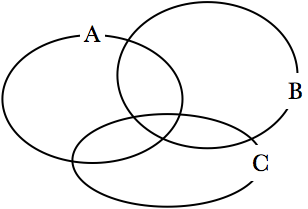
\includegraphics[scale=0.35]{FiguresMaths/3sets}
        \caption{Three sets, $A$, $B$ and $C$, in ``general" position, i.e., with all possible overlaps.}
        \label{fig:unionSetsInit}
\end{center}
\end{figure}
\begin{figure}[htb]
\begin{center}
        
\includegraphics[scale=0.35]{FiguresMaths/RuleAdditive}
        \hspace{1cm}
        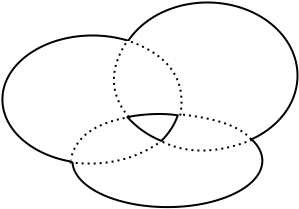
\includegraphics[scale=0.35]{FiguresMaths/RuleAdditive2}
        \caption{The union of sets $A$, $B$, and $C$ (left), and their intersections (right).}
        \label{fig:unionSets}
\end{center}
\end{figure}
In order to draw explicit expressions that express the content of  Fig.~\ref{fig:unionSets}, one must apply the Law of
{\em inclusion and exclusion} in multiple ways, as we compensate for the 
pairwise and triple intersections among  sets $A$, $B$, and $C$.  A careful reckoning using the figure 
indicates that
\[ |A \cup B \cup C| \ \ = \ \ 
\big(|A| + |B| + |C| \big) - \big( |A \cap B| + |A \cap C| + |B \cap C| \big) + |A \cap B \cap C|. \]
In particular, we begin by {\em including} the union; then we {\em exclude} the pairwise intersections, which
were double-counted; and we finally {\em include} the triple intersection, which was doubly excluded.

\item
{\em The multiplication rule} \index{The multiplication rule for counting elements of sets}

This rule tells us how to count the cardinalities of Cartesian products of sets, as
illustrated in Fig.~\ref{fig:cartesianproduct}.
\[ |A \times B| \ \ = \ \ |A| \cdot |B| \]
The multiplication rule extends immediately to multiplicities of sets; e.g., for three sets:
\[  |A \times B \times C| \ \ = \ \ |A| \cdot |B| \cdot |C| \]

As an important special case, we note that
\[ |A \times A \times \cdots  \times A| \ \mbox{ ($p-1$ times)}  \ \ = \ \ |A|^p \]
The exciting feature in this last equality is that the set
 \[ A \times A \times \cdots  \times A  \mbox{($p-1$ times)} \]
is a (nonstandard) way of representing the set of length-$p$ strings of elements of $A$.
Thereby, the multiplication rule gives us an alternative way to 
view---and to prove---Proposition~\ref{thm:b-ary strings}.
\end{itemize}

\bigskip

As we move forward, we shall encounter many other ways of counting the elements of sets,
most importantly by using operations involving {\it selection} and {\it rearrangement}.  As we
proceed with this new material, we will encounter old friends, often wearing new clothing.  We
will renew our acquaintance with the factorial operation and with binomial coefficients; we will
have cause to recall the pigeonhole principle in new settings.  And, we will discover new domains
of application, as we move beyond ``pure" mathematics to the applications of mathematical
laws in domains related to probability and statistics.
Let us begin our journey.

\subsection{Counting Based on Set Arrangement and Selection}
\label{sec:set-arrangement}

This section introduces the primary operations that are used for arranging finite sets as we
establish a base for studying combinatorial probability.  The importance of set-arrangement
in this context results from the common practice of defining
discrete probability/likelihood as a counting problem---most specifically, of defining the ratio:
\[ 
\frac{\mbox{number of ways of achieving a targeted event $E$}}{\mbox{number of possible events}}
\]
as the ``probability" of event $E$.

\medskip

We focus on three notions of arranging, and selecting from, a set of $n$ objects:
\[ \{ x_1, x_2, \ldots , x_n\} \]
When useful for explaining some idea, we sometimes identify the $x_i$ as some specific type
of objects, such as numbers, but generally we do not exploit any specific
characteristics of the $x_i$.

\medskip

\noindent {\it Permutations}.\index{permutation}
A permutation of an $n$-element set $A$ is a {\em fixed ordering} of the elements of $A$:  
each element of $A$ appears precisely once in the ordering.  We denote a permutation
of an $n$-element set via the notation
\[ (x_1,x_2, \ldots , x_n) \]
where each $x_i$ appears precisely once.  Note that we use parentheses for grouping,
as in ``$(3,2,1,4)$", instead of braces, as in ``$\{3,2,1,4\}$", to emphasize the ordering.  In
particular,
\[ \{3,2,1,4\} \ = \ \{1,2,3, 4\} \ \ \ \mbox{ but } \ \ \ (3,2,1,4) \ \neq \ (1, 2, 3,4) \]

\medskip

In terms of problems relating to {\em selecting}\index{selection problems}
$m$ elements from a set of $n \geq m$ elements, permutations give rise to the most demanding
genre of selection: {\em They demand accounting for both the {\em identities}
of the selected elements and the {\em orders} in which the elements were selected.}

\medskip

It is a straightforward exercise to count the number of permutations of $n$ items.

\begin{prop}
\label{thm:no-permutation}
The number of permutations, $P(n)$, of a $n$-element set equals $n!$
\end{prop}

\begin{proof}
Just for the practice, we describe two inductive proofs of this simple result, based on two
quite-distinct eays of constructing permutations.  We merely
sketch the inductions underlying the proofs, leaving details for your practice.

\medskip

\noindent {\bf 1.}
To construct a permutation of the $n$-element set $\{ x_1, x_2, \ldots , x_n\}$:
\begin{itemize}
\item
Select the first element of the permutation in $n$ ways: any $x_i$ will work.
\item
Having selected the first item, we are left with the $(n-1)$-element version of the problem.
\end{itemize}
We thereby find that $P(n)$ is specified recursively as follows.
\[
P(n) \ = \ \left\{
\begin{array}{cl}
1 & \mbox{ if } \ n=1 \\
n \times P(n-1) & \mbox{ if } \ n>1
\end{array}
\right.
\]
By elementary reasoning, we find that $P(n) \ = \ n!$.

\bigskip

\noindent {\bf 2.}
To construct a permutation of the $n$-element set $A = \{ x_1, x_2, \ldots , x_n\}$:
\begin{itemize}
\item
Assume, inductively, that you are given a fixed 
permutation $(x_1, \ldots , x_{n-1})$ of an $(n-1)$-element subset $A'  \subset A$,
chosen somehow from among the $(n-1)!$ possible orderings of set $A'$.  (Note
the thinly veiled use of induction.)
\item
Take element $x_n$, which does not belong to $A'$, and place it into the ordering of $A'$
that you are given.  You can place $x_n$ in any of $n$ positions in the new permutation:
  \begin{itemize}
  \item
before (i.e., to the left of) all of the preplaced elements of $A'$;
  \item
after (i.e., to the right of) all of the preplaced elements of $A'$;
  \item
in between any adjacent preplaced elements of $A'$.
  \end{itemize}
Each of the preceding $n$ choices creates a unique permutation of the $n$-element set $A$.
\end{itemize}
Using arithmetic virtually identical to case {\bf 1} verifies that $P(n) \ = \ n!$.

\medskip

\noindent
Other variants on the preceding proof themes will undoubtedly occur to you.   \qed
\end{proof}


%%%%%%%%%%%%%%%%%%%%%%%

\medskip

\noindent {\it Combinations}.\index{combination}
Within the context of selection problems, combinations are the ``next step down" in
strictness from permutations.  When one selects $m$ items from a set of $n \geq m$ items,
combinations are concerned with the {\em identities} of the elements selected, but not with 
the order in which they elements are chosen.

\noindent (This willingness to ignore order gives a big hint about how to count the number of
combinations of $m$ items chosen from $n$.  Can you figure out how to use the hint before
we get to Proposition~\ref{thm:no-combination}?)

\medskip

Factorials play as essential a role in combinational selection as in permutational selection, but
now it plays a {\em dual} role: choosing the identities of the selected elements {\em and} factoring out
the order in which the elements were selected.  The binomial coefficients that we introduced
in Section~\ref{sec:binomial-coeff} and that have arisen several times since then
throughout our journey are
(literally!) tailor made for this genre of selection problem.  Recall that
\[ {n \choose m} \ = \ \frac{n \times (n-1) \times \cdots \times (n-m)}{m!} \ = \  \frac{n!}{m!(n-m)!} 
\]

\begin{prop}
\label{thm:no-combination}
The number of ways of selecting $m$ elements from a set of $n \geq m$ elements, while 
ignoring the order in which the $m$ elements were selected is $\displaystyle {n \choose m}$.
\end{prop}

\begin{proof}
The number of {\em ordered} ways of selecting $m$ elements from a set of $n \geq m$
elements is 
\begin{equation}
\label{eq:combination}
n \times (n-1) \times \cdots \times (n-m+1) \ = \ \frac{n!}{(n-m)!}
\end{equation}
To wit: One can select the first element in any of $n$ ways.  Having selected this element,
there are $n-1$ ways to choose the second element---and $n-2$ ways to choose the third
element, $n-3$ ways to choose the fourth element, and so on.

This method of numeration accounts for both the identity of the $i$th chosen element 
{\em and} the fact that it was the $i$th element chosen.  In other words, if element $x_1$
is the first element chosen,
and element $x_2$ is the second one chosen, then the two orders of selection
\[ x_1, \ x_2, \ \mbox{(a fixed order for the remaining $m-2$ selections)} \]
and 
\[ x_2, \ x_1, \ \mbox{(a fixed order for the remaining $m-2$ selections)} \]
are counted as separate events.  Easily, this overcounting uniformly expands each of the
events that we {\em do} want to account for by the factor $m!$, for this is the number of orders 
in which we could have selected the finally chosen $m$ elements.
 
This reasoning indicates that we can compensate for our overcounting by dividing the 
{\em ordered} tally (\ref{eq:combination}) by $m!$.  This compensation replaces tally
(\ref{eq:combination}) by $\displaystyle {n \choose m}$, whence the result.  \qed
\end{proof}

\medskip

\noindent \fbox{
\begin{minipage}{0.95\textwidth}
Binomial coefficients have made yet another appearance in our journey!  The many situations
that are counted by this construct are only suggested by their occurrence here, in respect to
probabilities, as well as in Chapter~\ref{ch:Summation} within the context of evaluating 
summations and in Chapter~\ref{ch:Recurrences} within the context of solving recurrences.  
The multiple occurrences of binomial coefficients within these apparently unrelated contexts 
provide a powerful argument for the value of abstracting beyond the superficial details of 
phenomena in the direction of their deep essentials.  This insight will only be reinforced as 
we proceed with our study of combinatorial probabilities.
\end{minipage}
}

\bigskip

\index{derangement}

\noindent {\it Derangements}.
Derangements represent one of the simplest forms of {\em avoidance problems}.  Here is a
well-known version of such a problem, in preparation for the general definition.

Professor $X$ views it as a win-win strategy for the students in her class to grade each
others' essays on {\it The Essential Truth in the Universe}.  The essays thereby get graded faster,
as the grading process becomes a parallel rather than sequential computation.  Moreover,
each student gets a chance to see how another student has interpreted some basic
component of the human experience.  The only complication is: How should Professor $X$ 
allocate essays among her students.  {\em The process must ensure that no student is assigned her
own essay to critique.}

The challenge that Professor $X$ is facing is known as a {\em derangement problems}.

\medskip

\noindent {\em
A {\em derangement} of a (finite) set $A$ is a {\em bijection} $f: A \leftrightarrow A$ that has no 
{\em fixed point}.}  In other words, for every $a \in A$, we must have $f(a) \neq a$.

\medskip

Clearly, derangements always exist.  One can just number the elements of set $A$ by the numbers
$0, 1, \ldots, |A|-1$ and specify $f(a) = a+1 \bmod |A|$.

But, playing around with some sets should convince you that derangements are not so common!
In fact, the set  $A = \{0, 1,2 \}$ admits $6$ self-bijections, but only two are derangements, namely:
\[
\begin{array}{lll}
f(a) = a+1 \bmod 3 &: \mbox{which maps} &(0 \rightarrow 1),  (1 \rightarrow 2), (2 \rightarrow 0) \\
\mbox{and} &  & \\
g(a) = a-1 \bmod 3 &: \mbox{which maps} & (0 \rightarrow 2),  (1 \rightarrow 0), (2 \rightarrow 1)
\end{array}
\]
How many derangements does an arbitrary $n$-element set $A$ have?   We denote this quantity
by $d(n)$.  While we leave most study of the non-elementary topic of derangements to the reader,
we do derive a recurrence for $d(n)$. 

\medskip

We compute $d(n)$ for arbitrary $n \in \N^+$ via the following recursion:
\begin{itemize}
\item
For $n=1$:  \ $d(1) = 0$.

To wit, the unique bijection in this case consists only of a fixed point. 

\item
For $n=2$:  \ $d(2) = 1$.

To wit, there are two bijections in this case, the identity, which has two fixed points, and the swap,
which is a derangement.

\item
For $n > 2$: \ $d(n) = (n-1) (d(n-1) + d(n-2))$:

To wit: In any derangement, the first element of $A$, call it $a$, must map to some $b \neq a$.  There
are $n-1$ ways in which $b$ can be chosen.

\begin{itemize}
\item
There are $d(n-2)$ derangements under which element $b$ maps to $a$.  In detail, we know
everything about $a$ and $b$, so the remaining $n-2$ elements of $A$ can ``derange" in all
possible ways.

\item
There are $d(n-1)$ derangements under which element $b$ does not map to $a$.  In detail,
as the process of ``choosing an image" passes through $A$, every element has two forbidden
choices: it cannot choose itself (or these would be a fixed point) and it cannot choose one other
element (for element $b$, this is element $a$).  In some sense, the notion of a
forbidden element gets passed around, changing its identity at every step.
\end{itemize}
%$d(n) = (-1)^n + n d(n-1)$
\end{itemize}

\medskip

Interestingly, as the sizes of the sets of interest number of objects grows without bound, the
proportion of bijections that are derangements tends to the limit $1/e$, where $e$ is Euler's
constant (the base of natural logarithms).

\ignore{***********
bability that none appears in its correct position approaches
$p=lim_{n \rightarrow \infty}\frac{d(n)}{n!}=\frac{1}{e}$. 

{\Denis Interesting: to be detailed in more details...}
*****************}


\section{Introducing Combinatorial Probability via Examples}
\label{sec:combinatorial-prob}

Perhaps the easiest and most engaging way to introduce ``combinatorial
probability''---i.e., probability via counting"---is by calculating
game-related likelihoods---deals of cards, rolls of dice, and guessing
games of various sorts.  ``Why is one specific genre of deal in poker
(say, a straight) worth more than another (say, three of a kind)?"
The arithmetic required for such a discussion is elementary, and the
references to ``{\it gedanken} gambling'' are easily understood and
are of some interest even to non-gamblers.  One can also introduce in
such a setting concepts such as randomness, bias, etc., that are so
important in the design of experiments and the analysis of their
outcomes.

This, then, will be our approach to the subject of combinatorial probability.  The reader has already
seen more than enough ``dry" facts about sets and how to count their elements.  It is time to
reap the rewards of acquiring access to that material. 

\ignore{***************
\subsection{A Practical Introduction to Probability}
\label{sec:prob-stat}

Elements of probability theory and statistics infuse every area of
computing.  The practicality of many algorithms that are
experientially the most efficient for their target tasks depend on the
{\em distribution} of inputs in ``real" situations.  Design
methodologies for crucial complex circuits must acknowledge the {\em
  mean times to failure} of the critical components of the circuits.
Sophisticated searching algorithms must take into account the relative
{\em likelihoods} of finding one's goal in the various optional search
directions.  Analyzing and understanding large corpora of data
requires a variety of methodologies that build on the concepts of {\em
  clustering} and/or {\em decomposition}.

A student needs at least an introduction to the foundations of
probability and statistics to even understand, all the more so to
master, the terms highlighted in the preceding paragraph.  We outline
many of the key concepts that a student must be exposed to in the
following subsections.

{\Denis Here we may be more precise about the content: the probabilities are built upon combinatoric rules, another interesting point is to distinguish between probability and statistics...}
*****************}

Before we begin to play, though, we establish some expectations,
beginning with the combinatorics-based definition of ``probability''
that sets the tone for this section.

\bigskip

\noindent
{\em  The (discrete) {\em probability}, or, {\em likelihood}, of an event is the ratio:}
\begin{equation}
\label{eq:prob-def-ratio}
\frac{\mbox{number of targeted events}}{\mbox{number of possible events}}
\end{equation}

\noindent
This approach to probabilities has important technical consequences.
  \begin{itemize}
  \item
The probability of any targeted event $E$ is $\leq 1$.  This means:
    \begin{itemize}
    \item
If the probability of $E$ is $1$, then event $E$ is a certainty.
    \item
If the probability of $E$ is $< 1$, then event $E$ is possible but not certain.
   \end{itemize}

 \item
The probability of any targeted event is $\geq 0$.   This means:
    \begin{itemize}
    \item
If the probability of $E$ is $0$, then event $E$ is an impossibility.
    \item
If the probability of $E$ is $> 0$, then event $E$ is a possibility.
   \end{itemize}

  \item
The more likely an event is, the closer its probability is to $1$.
  \item
By the addition rule for counting sets, the joint probability of two {\em disjoint} events
equals the sum of the events' probabilities.
  \item
As a special case of the preceding rule: the joint probability of two {\em complementary} events
equals $1$.  This is because the complement of an event whose probability is $p$ has
probability  $(1-p)$.
  \end{itemize}

\bigskip

\noindent \fbox{
\begin{minipage}{0.95\textwidth}
As just asserted, we view a probability as a number $p$ in the range $0 \leq p \leq 1$.  
It is also very common, though, to view a probability as a {\em percent}, as in

\smallskip

\hspace*{.2in}``The likelihood of rain this morning is $50$\%."

\smallskip

In order to understand these competing locutions, the reader should recall that the word
``percent" derives from the Latin ``{\it per centum}", which means ``per hundred".
Therefore, one can always interchange the following  locutions

\smallskip

\hspace*{.2in}``Event $E$ occurs with probability $p$."

\hspace*{.2in}``Event $E$ occurs with probability $(100 p)$\%."
\end{minipage}
}

\bigskip

\noindent
We are going to focus on {\em games of pure chance}---with no
complicating notion of strategy---because our underlying interest is in
probability, not game theory.

\bigskip

\noindent \fbox{
\begin{minipage}{0.95\textwidth}
There exists an exciting mathematical field of study that is dedicated to all games:
games of pure chance (which is our focus), games that combine skill and chance (e.g.,
backgammon, bridge, or poker), and games of pure skill (e.g., chess or GO).   But, alas,
the issues one must deal with when studying the broad spectrum of games go beyond the 
scope of our introductory text.

\index{von Neumann, John} \index{Morgenstern, Oskar} \index{Nash, John}
We recommend to the reader just two classics works that may be of interest for historical 
and cultural reasons, as well to supply a foundation for further study.  The first reference is to the
classic \cite{vonNeumann-Morg} by American polymath John von Neumann 
and German economist Oskar Morgenstern, which established the
connection between the mathematical subject of game theory and the field of economics.  
(Now-familiar concepts such as ``rational game" and ``zero-sum game" originated in
\cite{vonNeumann-Morg}.)  The second classic is \cite{Nash50}, by the American mathematician
John Nash, which introduced the now-familiar notion of ``Nash equilibrium."
(The story behind \cite{Nash50} was movingly related in the movie ``{\it A Beautiful Mind}".)
\end{minipage}
}


\subsection{The Game of Poker: Counting Joint Events}

We focus on a typical deck of 52 playing cards: The cards are partitioned into

\medskip

\noindent
\begin{tabular}{cll}
$*$ &
four {\em suits}:  & {\sc clubs}, {\sc diamonds}, {\sc hearts}, {\sc spades} \ (in increasing value) \\
  \\
$*$ &
$13$ {\em face values}: &
$\displaystyle \left\{
\begin{array}{l}
\mbox{number cards}: 
2, 3, 4, 5, 6, 7, 8, 9 \\
\mbox{picture cards}: 
\mbox{{\sc Jack, Queen, King, Ace}  (in increasing value)}
\end{array}
\right.$ 
\end{tabular} 

\medskip

\noindent
In a popular version of the game of poker, each player is dealt a {\it hand} consisting of five cards.
The total number of possible $5$-card hands, i.e., of (unordered sets) of $5$ cards, is just the number
of ways of choosing a $5$-element set from a $52$-element set.  Using the counting techniques from
Section~\ref{sec:set-arrangement}, we discover that this ``astronomical" number is
\index{the number of random $5$-card deals in poker} 
\[
{32 \choose 5} \ \ = \ \ \frac{52!}{5! 47!} \ \ = \ \ 2,598,960 
\]
The size of this number explains much of what of makes the game of poker so interesting.

\medskip

Of course, it is the {\em patterns} of the cards in various hands that determines which hands
beat other ones in the competition that is at the heart of poker.  It is a reasonable
conjecture that the {\em value} of a given pattern is proportional to the {\em likelihood}
of that pattern's arising in a random deal of five cards.  (Of course, {\em random} deals are 
the personification of a {\em fair} game.)

We now calculate the likelihoods of a variety of patterns arising in a fair game, in order to study
the validity of the preceding conjecture.  As we derive the likelihoods of the various patterns,
observe the many invocations of the multiplication rule for the probabilities of independent events.

\medskip

\index{royal flush (in poker)} \index{straight flush (in poker)}
\begin{itemize}
\item
A {\it royal flush} is a poker hand of the form

\hspace*{.25in}$10$, \ {\sc Jack}, \ {\sc Queen}, \ {\sc King}, \ {\sc Ace} \ \ of the same suit

\noindent
There are only four ways to form a royal flush---one for each suit.  Therefore, the probability that
a fair deal will produce such a hand is
\[ 
Pr(\mbox{royal flush}) \ \ = \ \
\frac{4}{2,598,960} \ \ = \ \ {1 \over {649,740}} \ \ \approx \ \ 0.00000154 \ \ = \ \ 1.54 \times 10^{-6} \]

\item
A {\it straight flush} is a poker hand in which the cards share the same suit and follow one 
another in value.  Thus, a royal flush is a straight flush whose highest-rank card is an {\sc Ace}.

Let us calculate the number of straight flushes that are {\em not} royal flushes.

The counting is similar as for a royal flush:  For each suit, there are nine sequences of $5$ cards
that are consecutive in rank.  From lowest rank to highest:
\[ \begin{array}{llccccc}
\mbox{Hand \#1}: & &
2 & 3 & 4 & 5 & 6 \\
\mbox{Hand \#2}: & &
3 & 4 & 5 & 6 & 7 \\
\mbox{Hand \#3}: & &
4 & 5 & 6 & 7 & 8 \\
\mbox{Hand \#4}: & &
5 & 6 & 7 & 8 & 9 \\
\mbox{Hand \#5}: & &
6 & 7 & 8 & 9 & 10 \\
\mbox{Hand \#6}: & &
7 & 8 & 9 & 10 &  \mbox{J} \\
\mbox{Hand \#7}: & &
8 & 9 & 10 &  \mbox{J} &   \mbox{Q} \\
\mbox{Hand \#8}: & &
9 & 10 &  \mbox{J} & \mbox{Q} &  \mbox{K}  \\
\mbox{Hand \#9}: & &
10 &  \mbox{J}
     & \mbox{Q}
     & \mbox{K}
     & \mbox{A}
\end{array} \]
The probability of being dealt a royal flush is, thus, precisely $1/9$ the probability of being dealt a
straight flush.  The probability of getting a straight flush is, therefore,
\[  Pr(\mbox{straight flush}) \ \ = \ \
{3 \over {216,580}} \ \ \approx \ \ 0.0000139  \ \ = \ \ 1.39 \times 10^{-5} \]

\item
{\it Four-of-a-kind} is a poker hand of the form \\
\hspace*{.25in}$X, \ X, \ X, \ X, \ Y$ \\
where $X, Y \in \{2, \ 3, \ 4, \ 5, \ 6, \ 7, \ 8, \ 9, \ \mbox{J}, \ \mbox{Q}, \ \mbox{K}, \ \mbox{A}\}$, 
and $X \neq Y$.
\index{four of a kind (in poker)}

\medskip

There are $13$ possible face values; each is a candidate for being card $X$.  Having chosen card
$X$, there are $48$ possible choices for card $Y$.  Each selection  of
cards $X$ and $Y$ specifies a unique {\it four-of-a-kind} poker hand.
The multiplication principle thus tells us that there are precisely $13 \times 48 = 624$
{\it four-of-a-kind} poker hands, so the probability of being dealt such a hand is
\[ 
Pr(\mbox{four of a kind}) \ \ = \ \
\frac{624}{2,598,960 }  \ \ \approx \ \ 2.4 \times 10^{-4} . \]

\ignore{***********
is a remaining card left that is any one among the 48 remaining ones.
Indeed, according to the multiplicative principle, it remains ${12 \choose 1}$ in each of the $4$ colors. 
Thus, $13 \times 48 = 624$, which corresponds to the probability $0.00256$.
*************}

\item
We finally look at two more poker hands together because the analyses of their
respective patterns are so similar.
\begin{itemize}
\item
A {\it Full house} is a poker hand of the form \\
\hspace*{.25in}$X, \ X, \ X, \ Y ,\ Y$ \\
where $X, Y \in \{2, \ 3, \ 4, \ 5, \ 6, \ 7, \ 8, \ 9, \ \mbox{J}, \ \mbox{Q}, \ \mbox{K}, \ \mbox{A}\}$, 
and $X \neq Y$.
 \index{full house (in poker)} 

\medskip

\index{three of a kind (in poker)}
\item
{\it Three of a kind} is a poker hand of the form \\
\hspace*{.25in}$X, \ X, \ X, \ Y, \ Z$ \\
where $X, Y,  Z \in \{2, \ 3, \ 4, \ 5, \ 6, \ 7, \ 8, \ 9, \ \mbox{J}, \ \mbox{Q}, \ \mbox{K}, \ \mbox{A}\}$, 
and $|\{X, Y, Z\}| =3$.  The final equation here  is a ``cute", succinct, way of saying that $Y$ and $Z$
differ both from $X$ and from each other.
\end{itemize}
For both of these patterns, the analysis begins by noting that the face-value $X$ can be chosen
in $13$ ways.  Having chosen face-value $X$, we select three of the four cards with that face-value:
this choice can be made in $\displaystyle {4 \choose 3}$ ways.  The $X$ component of the hand
has now been selected.

With the {\it full-house} pattern, we must now choose the face-value $Y$.  This can be done in $12$ ways.
The selection of the hand is completed once we select the $\displaystyle {4 \choose 2} = 6$
needed cards that have face-value $Y$.

Summing up, the {\it full-house} pattern can be assembled in
\[ 13 \cdot {4 \choose 3} \cdot 12 \cdot {4 \choose 2} \ \ = \ \  3,744 \]
ways, so the probability of being dealt such a hand is
\[ 
Pr(\mbox{full house}) \ \ = \ \
\frac{3744}{2,598960}  \ \ \approx \ \ 1.44 \times 10^{-3} . \]

\medskip

To finish up the {\it three of a kind} poker hand, we remark that once we have selected the $X$
component of the hand,  we must select the remaining cards by choosing the (distinct) face-values of
$Y$ and $Z$; this can be done in $\displaystyle {12 \choose 2} = 66$ ways.  Then, for each of these
choices we must select a specific card, which can be done in $4$ ways.  We thereby find that the
{\it three of a kind} pattern can be assembled in
\[ 13 \cdot {4 \choose 3} \cdot {12 \choose 2} \cdot 4^2 \ \ = \ \  54,912 \]
ways, so the probability of being dealt such a hand is
\[ Pr(\mbox{three of a kind}) \ \ = \ \
 \frac{}{2,598,960}  \ \ \approx \ \ 2.11 \times 10^{-2} . \]

\ignore{****************
The analysis of the first of these two patterns follows the same logic as for the Four-of-a-kind.
Again, there are as many possibilities of the $3$ base cards of the pattern than the number of cards in a color ($13$)
with only $3$ colors among the 4: ${4 \choose 3}$.
The two remaining cards should be different from the kind (and different from each other), 
thus, their number is to select $2$ among the $12$ remaining ones,
each one can take any colors (their number is $4^2$).
The final expression is:

$13.{4 \choose 3}.{12 \choose 2}.4^2 = 858$

For getting a Full House, the enumeration is close to the previous one, but there is a slight difference 
on the two remaining cards,
which here should by a pair (two of the same kind, that is only $1$ card among the $12$, 
this card can take any of the four colors),
thus:
\[ 13 \times {4 \choose 3} \times {12 \choose 1} \times 4 = 156 \]
**********************}
\end{itemize}

One can find in many sources (such as the Internet) tables that: enumerate all possible poker hands,
describe all ways of assembling each hand, and compute the probabilities of being dealt each hand.
Of course, our interest has been in exposing how to perform these calculations, not with their
results---but it s fun to see why the various poker hands have their relative values in the game.



\subsection{The Monty Hall Puzzle: {\em Conditional} Probabilities}
\label{sec:monty-hall}

The following real-life situation illustrates that reasoning
probabilistically is not easy and can be quite unintuitive.

We recall a popular tv show from the 1970s and 1980s, \textit{Let's
  Make a Deal}.\index{Let's Make a Deal} In one segment of each airing of the show, a
contestant was confronted by three doors, door (1), door (2), and door
(3); see Fig.~\ref{fig:MonthyHal-1}.
\begin{figure}[htb]
\begin{center}
        \includegraphics[scale=0.4]{FiguresMaths/MonthyHallInitial}
%            \includegraphics[scale=0.5]{FiguresProba/MonthyHallInitial}
        \caption{The three doors of \textit{Let's Make a Deal}.}
        \label{fig:MonthyHal-1}
\end{center}
\end{figure}
The contestant was told that a jackpot was behind one of the doors;
the other two hid less-desirable prizes.  The show's host, Monty Hall,
invited the contestant to choose one of the doors:
she would receive whatever prize was behind the door she selected.
\index{Hall, Monty} 

Since the door names are irrelevant to the story, let us assume that
the contestant chose door (1).  Before that selection was considered
final, Monty Hall would open {\em one of} doors (2) or (3), i.e., one
of the two {\em unchosen} doors.  Again for illustration, let us
assume that Monty opened door (3).  Assuming that the jackpot did {\em not} appear 
behind door (3), Monty now gave the contestant the
option of changing her initial choice, from door (1) to door (2).

What should the contestant do?  

Let us begin with intuition.  As the story began, the contestant had a
one-in-three chance of choosing the door that hid the jackpot.  As the
story progresses, is it conceivable that these odds could have changed after door
(3) is shown {\em not} to hide the jackpot?  How could this be?

\index{von Savant, Marilyn}
Well, the popular (well-named) columnist Marilyn von Savant
published an analysis that shows that {\em it is better to change one's choice!}  
Here is her reasoning, enhanced by the illustration in Fig.~\ref{fig:MonthyHall-2}.
\begin{figure}[htb]
\begin{center}
        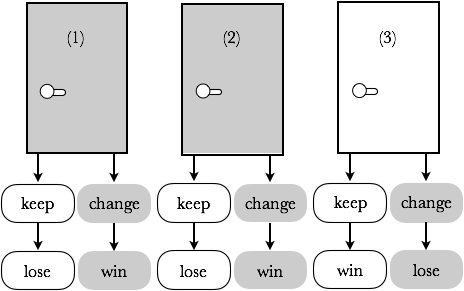
\includegraphics[scale=0.4]{FiguresMaths/MonthyHall}
%                \includegraphics[scale=0.4]{FiguresProba/Monthy}
        \caption{Suppose the jackpot is behind door (3). 
        If we select it, we lose if we change the initial choice.
        However, it is better to change if we select one of both other doors (1) or (2).}
        \label{fig:MonthyHall-2}
\end{center}
\end{figure}
We distinguish the two possible cases.
\begin{itemize}
\item
If the contestant had selected the jackpot-door at the beginning, then
holding on to this choice leads to the same probability of success as
she had from the beginning, namely, {\em one-third}.
\item
If the contestant had selected a wrong door at the beginning---which
occurs with probability {\em two-thirds}---then she will win the
jackpot if she now changes her initial (erroneous) choice.
%because now the choice in among two cases. 
\end{itemize}
Thus, quite unintuitively, the contestant should change her original
choice based on the information she has now.

\smallskip

You can have fun by confronting your friends with this unintuitive analysis.

\medskip

\index{conditional probability} \index{Bayes's Theorem}
Of course, this is not just a trick!  It is a demonstration that you can improve your chances 
of winning by taking advantage of all available information!  The ``science'' behind this 
analysis is built upon the topic of {\em conditional probability}, in general, and Bayes's 
Theorem, in particular.  Both topics are beyond the scope of this text: See \cite{Lee12} for 
a general presentation of this topic, and see \cite{Bayes} for the original work.

And---see the interactive sites on the Internet that actually perform the
computation of likelihoods!


\subsection{The Birthday Puzzle: {\em Complementary} Counting}
\label{sec:birthday-puzzle}
\index{birthday puzzle}

This section presents another application of the rules of enumeration
to the calculation of probabilities.%~\cite{DumasTrystram}.
The main message with this application is:
{\em it is sometimes easier to calculate the probability that an event {\em does not} occur than
the probability that it {\em does} occur.}  (Of course, this is a ``rule of thumb", not a formal 
proposition. But, we do invite you to replicate the conclusions of this section via a direct argument.)

\medskip

A common technique that teachers employ to establish rapport with a new class is to determine 
whether any students in the class share a birthday.  We demonstrate in this section that when 
the class has (at least) around 30 students, the answer is usually \textit{yes}.  The fact that we 
can make such a specific claim  suggests that the presence of birthday-sharers is not a mere 
accident---there are probabilities at work here!

\smallskip

Let us study the following question.

\smallskip

{\it How many people must gather before the probability that some two share}

{\it a birthday reaches 50\%?}

\medskip

\ignore{****************
\noindent \fbox{
\begin{minipage}{0.96\textwidth}
If the teacher's new class focuses on a mathematical subject, then there is a teaching
opportunity here!  The teacher and the students can collaboratively derive an answer
to the preceding question.
\end{minipage}
}

\bigskip
***************}

\noindent
We now develop an answer to the birthday-sharing question, based on the assumption
that all dates are equally probable as potential birthdays.

\bigskip

Let us focus on a common year, with 365 days; a simple modification of the coming calculation 
accommodates leap years.  A first, obvious, remark is that when there are 366 people in the 
class---and only then---the pigeonhole principle {\em guarantees} (with probability 100\%) 
that some two people share a birthday.  When we lower our birthday-sharing target to a 
{\em 50\% probability} of a shared birthday, how much does this lower the required population 
of 366?  Somewhat unintuitively, the required number is lowered dramatically!

\bigskip

\index{dual problem} 
We simplify the calculational component of our solution considerably by focusing on the 
{\em dual} form of our problem.  That is:

\smallskip

\noindent {\em Instead of} determining a {\em lower bound} on the population
that would guarantee a 50\% probability of a shared birthday,

\noindent {\em we determine} an {\em upper bound} on the population that would
guarantee a 50\% probability of {\em no} shared birthday.

\medskip

Since we assume that all birthdays are equally likely, the probability
that any particular person has any particular birthday is $1/365$.  In
other words, the space of all possible assignments of birthdays to all
$n$ people has $365^n$ assignments---all of which are equally likely.

Let us perform the following {\em gedanken} experiment (i.e., ``thought-experiment").

\smallskip

Say that we have an assemblage of $n$ ``proto-people"---i.e., people who do not yet have  birthdays.
Our task is to assign birthdays to these folks in such a way that no two of them share a birthday.

Focus first on person \#1: her birthday can be selected from any of
the $365$ (indistinguishable) days of the year.  Moving on to person
\#2: his birthday can be selected only from the $364$
(indistinguishable) days of the year that person \#1 has not
``chosen'': otherwise persons \#1 and \#2 would share a birthday!  By
similar reasoning, person \#3's birthday can be selected from only the
$363$ days that the first two people have not claimed, person \#4
chooses from among $362$ days, and so on, until person \#$n$ chooses
from among $365-(n-1)$ days.

The preceding tally indicates that among the $365^n$ possible
assignments of birthdays to $n$ people, only
\[ 365 \times 364 \times 363 \times \cdots \times
(366-n+1) \ = \ \frac{365!}{(365-n)!} 
\]
assignments have no two people sharing a birthday.  Worded as a
probability, then, if we denote by $p(n)$ the probability that there are no shared
birthdays in a population of $n$ people, we find that
\begin{eqnarray*}
p(n) & = &
\frac{\mbox{number of birthday assignments with no shared birthday}}
{\mbox{total number of birthday assignments}} \\
 &  = & \frac{365!}{ (365-n)!  \times 365^n} \\
 & = & \frac{n!}{365^n} {365 \choose n}
\end{eqnarray*}

\medskip

Let us return to our original problem, which focuses on assignments in
which there exists at least one shared birthday.  Since the event \\
\hspace*{.25in}some two people share a birthday \\
is the complement of the event \\
\hspace*{.25in}no two people share a birthday \\
the probability of a shared birthday is precisely $1-p(n)$.  We find
that for $n=23$, the desired probability is $0.5073$:  In other words,

\begin{prop}
In any group of $23$ people, the likelihood that two people share the same
birthday is slightly greater than $50\%$, assuming a year with $365$
equally likely days.
\end{prop}

When our teacher's class grows to 30 students, the probability of a shared birthday grows
to $70.632\%$.


\subsection{Sum-of-Spots Dice Games: Counting with Complex Events}
\label{sec:three-dice}
\index{Dice games}

Archaeology suggests that games have fascinated our species since our origins.  The 
games that have endured span a broad spectrum, from those that depend almost entirely 
on thinking and strategy to those that depend on pure chance.  (One would place chess 
at one end of this spectrum and (fair) flipping of a fair coin at the other end.)  A number of 
ancient games that have endured involve the rolling of 6-sided dice, each die\footnote{The 
word ``dice'' is plural.  The singular form is ``die''.}~having distinct numbers (usually denoted
by {\it spots}) on its six faces.  For convenience, we refer to each die's face-numbers via the 
numerals $1, 2, 3, 4, 5, 6$.  (Ancient Egyptians played such games, as did Roman legionaries; 
and such games persist in present-day casinos.)

\index{Dice games!craps} \index{Dice games!sum-of-three} 
We discuss two ancient dice games: The first game, known as ``{\it craps}'' in North America, 
involves rolling two dice at a time; the second game, which we call ``{\it sum-of-three}'',
involves rolling three dice at a time.  With both games, the outcome of interest is the {\em sum} 
of the spots on the upward-oriented faces of the rolled dice.  (For example, the sums
``$7$'' and ``$11$'' are winning outcomes in craps; ``$2$'', ``$3$'', and ``$12$'' are losing 
outcomes; all other sums are ``roll-again'' outcomes.)  We highlight the word ``sum'' to 
stress that the order in which the dice reveal their spots is not relevant.  This means that the
outcomes we distinguish consist of pairs of the form $ab$ for the game
craps and triples of the form $abc$ for the game sum-of-three, where:
\begin{itemize}
\item
each of $a, b, c$ is an integer from the set $\{1, 2, 3, 4, 5, 6\}$
\item
$ a \leq b \leq c$.  This is just a convenient way of saying that the
  order in which the numbers appear is irrelevant.
\end{itemize}
We call each such pair (in craps) or triple (in sum-of-three) a {\it configuration}.

Under the assumption of a {\em fair} game---i.e., one in which all
faces of all dice are equally likely to appear---we can analyze both
craps and sum-of-three by enumerating the $21$ possible outcomes of a
roll in the game of craps and the $56$ possible outcomes of a roll in
the game of sum-of-three; see Fig.~\ref{fig:dice-outcomes}.
\begin{figure}[htb]
\begin{center}
\begin{tabular}{ccc}
\begin{tabular}{|c|c|c|r|}
\hline
   &    &    & sum \\
\hline
11 &    &    & 2 \\
12 &    &    & 3 \\
13 & 22 &    & 4 \\
14 & 23 &    & 5 \\
15 & 24 & 33 & 6 \\
16 & 25 & 34 & 7 \\
26 & 35 & 44 & 8 \\
36 & 45 &    & 9 \\
46 & 55 &    & 10 \\
56 &    &    & 11 \\
66 &    &    & 12 \\
\hline
\end{tabular}
  &
\hspace*{.5in}
  &
\begin{tabular}{|c|c|c|c|c|c|r|}
\hline
 & & & & & & sum\\
\hline
111 & & & & & & 3\\
112 & & & & & & 4\\
113 & 122 & & & & & 5 \\
114 & 123 & 222 & & & & 6 \\
115 & 124 & 133 & 223 & & & 7\\
116 & 125 & 134 &  224 & 233 & & 8\\
126 & 135 & 144 & 225 & 234 & 333 & 9\\
136 &  226 & 145 & 244 & 235 & 334 & 10\\
146 & 236 & 155 & 245 & 335 & 344 & 11\\
156 & 246 & 336 & 255 & 345 & 444 & 12\\
166 & 256 & 346 & 445 & & & 13\\
266 & 356 & 446 & 455 & & & 14\\
366 & 456 & 555 & & & & 15\\
466 & 556 & & & & & 16\\
566 & & & & & & 17\\
666 & & & & & & 18\\
\hline
\end{tabular}
\end{tabular}
\end{center}
\caption{The possible outcomes of craps (left) and of sum-of-three (right).}
\label{fig:dice-outcomes}
\end{figure}

\bigskip

As one might expect, the analysis of craps is very similar to, and
much simpler than, the analysis of sum-of-three.  Therefore, we provide
only the latter analysis here, leaving the analysis of craps as an exercise.

We develop the enumeration of sum-of-three in two distinct ways, in the hope of 
encouraging the reader to seek multiple ways to think about such enumerations.
\begin{enumerate}
\item 
Our first technique of enumeration lists the $16$ possible sums of a roll of the three 
dice and, for each, lists all possible configurations that yield that sum.

The $16$ possible sums arise from the fact that dice are
labeled with the integers $1, 2, 3, 4, 5, 6$, so the smallest possible
sum is $3$ (which occurs when all three dice show the number $1$), and
the largest possible sum is $18$ (which occurs when all three dice
show the number $6$).  All possible sums are listed in
Fig.~\ref{fig:dice-outcomes}(right).  The depicted table allows
us to easily compute that the probability of obtain the sum $6$ in a
roll of three dice is $p(6) \ = \ 4/56 \ = \ 0.071\cdots$; in other
words, we expect to observe this sum with just a bit more than $7\%$ of rolls.

\item 
A rather different way of enumerating sums is to partition
configurations $abc$ based on the number of distinct numbers in the
set $\{ a, b, c\}$.
\begin{itemize}
\item
At one extreme, there are six configurations in which $a = b = c$,
based on the six possible values on the face of a die.
\item
In the intermediate case, either $a=b$ or $b=c$ but the third value is
distinct.
  \begin{itemize}
  \item
The situation $a=b$ can occur in $5$ ways (we must leave room for
$c$).  For each way, $c$ can assume $6-a$ values (because $c$ is the
biggest value).  There are, therefore, $15$ such configurations.
  \item
The situation $b=c$ is the mirror image of the preceding situation,
hence engenders the same number of configurations.
  \end{itemize}

\item
Finally, when $a$, $b$, and $c$ are all distinct (but appear in
increasing order): $a$ can assume the values $1, 2, 3, 4$.  For each
choice of $a$, $b$ can assume the values $a+1, a+2, \ldots, 5$.  And,
for each choice of $b$, $c$ can assume the values $b+1, b+2, \ldots,
6$.  A simple calculation identifies $20$ configurations in which $a$,
$b$, and $c$ are all distinct.
\end{itemize}
Of course, we again identify $56$ possible configurations.
\end{enumerate}

\bigskip

To close this section, let us consider the variant of the game
sum-of-three in which the order of observing outcomes $a$, $b$, and
$c$ does matter.  To expose the difference this attention to order makes,
let us look again at the table in Fig.~\ref{fig:dice-outcomes}(right).
We note, focusing for illustration just on sum $6$, that three
different configurations produce this sum:
\begin{enumerate}
\item one die of each value $1$, $2$, $3$
\item two dice of value $1$ and one of value $4$
\item three dice of value $2$
\end{enumerate}
In contrast, if the order in which values occur matters, then the
sum $6$ arises in {\em ten} different ways.  Specifically, we now
roll the dice one at a time instead of as a group of three, and we
observe the sum $6$ arising in the ten ways enumerated in
Fig.~\ref{fig:dice-ordered-outcomes}; in this figure, each column
represents a roll of die \#1, then of die \#2, then of die \#3.
\begin{figure}[htb]
\begin{center}
\begin{tabular}{|l||c|c|c|c|c|c|c|c|c|c|}
\hline
First die & 1 & 1 & 4 & 1 & 1 & 2 & 2 & 3 & 3 & 2   \\

Second die & 1 & 4 & 1 & 2 & 3 & 3 & 1 & 1 & 2 & 2   \\

Third die & 4 & 1 & 1 & 3 & 2 & 1 & 3 & 2 & 1 & 2  \\
\hline
\end{tabular}
\end{center}
\caption{Achieving sum $6$ via {\em ordered} rolls of three dice}
\label{fig:dice-ordered-outcomes}
\end{figure}

\medskip

\begin{figure}[htb]
\begin{center}
\begin{tabular}{|l||c|c|c|c|c|c|c|c|}
\hline
Sum & 3, 18 & 4, 17 & 5, 16 & 6, 15 & 7, 14 & 8, 13 & 9, 12 & 10, 11  \\
\hline
number of configurations & 1 & 3 & 6 & 10 & 15 & 21 & 25 & 27  \\
\hline
\end{tabular}
\end{center}
\caption{Achieving all possible sums via {\em ordered} rolls of three dice}
\label{fig:dice-ordered-configs}
\end{figure}
We leave it to the reader to verify the table in Fig.~\ref{fig:dice-ordered-configs}, 
which gives the number of configurations that engender each possible sum (from $3$ to $18$) 
in the ordered-roll version of sum-of-three.  Note that each possible sum $k$ is engendered 
by the same number of configurations as is sum $21- k$.  ({\em Can you figure out why?})  
The total number of configurations is $6^3 = 216$; easily, this number is equal to
\[ 2 \times (1 + 3 + 6 + 10 + 15 + 21 + 25 + 27). \]

\bigskip

%{\Denis This result is amazing since the series grows like the sum of the first $n_{th}$ integers, except for the last ones which are truncated. This is probably possible to prove it!}

\noindent {\it Summing up.}
We have developed several examples which illustrate how to compute the probability of an event
(e.g., observing a ``heads" when tossing a coin) by taking the ratio of the number of favorable 
instances of the event divided by the number of all possible instances of the event.  (In this trivial
example, the probability is clearly $1/2$ when the coin is fair.)  This approach can be adapted to
situations defined by repeated occurrences of an event, such as repeated rolls of a  die or 
repeated tosses of a coin.  (Continuing the trivial example of coin tosses: the probability of 
``heads-then-tails" in two flips of a fair coin is $1/4$ .)

\bigskip

{\Arny I have to think about this.  I am not sure that I really understand the points you are making.}
Probabilities are typically used in two complementary ways.
\begin{itemize}
\item
One uses probabilities to help understand phenomena that one observes.  Two simple examples involves
rolls of a die and flips of a coin.  
\ignore{*******
kind of questions may be studied.
First, "how the probability of the occurrence of an event (like obtaining a $6$) is related to practical results?"
The second question is somehow the reverse: "If we run several times an experience of rolling dices, is it possible 
to infer the corresponding probability?".
*********}
It is easy to see that if a die is fair then in a long run of rolls of the die, one should see (roughly) equally
many $1$'s as $2$'s, \ldots, as $6$'s.  (Terminologically, these six events are \textit{equiprobable}:
$p(1)=p(2)=p(3)=p(4)=p(5)=p(6)$.) Indeed, this gives one access to a test for determining whether a die
is fair: Roll the die lots of times, and test whether one sees each result roughly $\frac{1}{6}$ of the time.
By similar reasoning, one can determine whether a coin is fair by tossing it many times and seeing 
whether one observes (roughly) equally many {\sc head}s as {\sc tail}s.

This use of probability is common: study the probability and then, deduce the future behaviors.
The second question is the main purpose of statistics that is developed in the next section.

\end{itemize}

% discuss Probability versus Statistics...

{\Denis We have to mention the links with the two other places where we discussed Binomial coefficients, recurrences and arithmetic, in this last case, we presented a question of computing the probability of getting 25 tails over 40 trials while flipping coins...}
{\Arny I believe that we have already stressed in a few places how many conceptual uses one can make of 
binomial coefficients.}


\section{Probability Functions: Frequencies and Distributions}
\label{sec:prob-distributions}

\index{probability!frequency function} 
\index{probability!sample space}
\index{probability!random variable} \index{sample space}
\index{random variable} 

Applications of probability theory usually operate with sets whose
elements represent the outcomes of individual moves in an
experiment---think, for instance of the deal of a single card or the
roll of a single die.  The range of possible outcomes is termes a {\it
  sample space}; and, a variable that ranges over the frequencies of
outcomes from the sample space is called a {\it random variable}.  The
goal of a probabilistic analysis is to capture important elements of
``{\em the truth}'', as exposed via experiments that produce sequences
of {\em outcomes}, each being an instantiaiton of a rendom variable
with a value from its sample space.

\subsection{Probability Frequency Functions and Related Measures}
\label{sec:prob-freq-fns+measures}

\subsubsection{Probability frequency functions}
\label{sec:prob-freq-fns}

Let us abstract the preceding environment, by focussing on:
\begin{itemize}
\item
a sequence $S = \langle s_1, s_2, \ldots, s_n \rangle$ of $n$ values
from an underlying sample space $\Sigma$.  Each value $s_i$ represents
one outcome of the $n$ produced by an $n$-trial experiment.

\smallskip

Exemplary sample spaces $\Sigma$:
  \begin{enumerate}
  \item
Rolls of a $6$-sided die: $\Sigma = \{1, 2, 3, 4, 5, 6\}$ .
  \item
The noontime temperatures observed in Grenoble, France:
$\Sigma = \{ t \ | \ -10 \leq t \leq 45\}$
  \item
The observed diameters of $n$ roller bearings after a given run at Factory $X$:
$\Sigma =$ the range of diameters of roller bearings.
\end{enumerate}

\item
a {\it frequency function} $f_S$ which reports on the multiplicity of each outcome
$s_i \in \Sigma$ within the sequence $S$.
  \begin{itemize}
  \item
For illustration, if 
\begin{equation}
\label{eq:sample-seq-10}
\Sigma \ = \  \{1, 2, 3, 4\} \ \ \ \mbox{ and } \ \ \
S \ = \ \langle 1, 2, 2, 3, 3, 3, 4, 4, 4, 4 \rangle
\end{equation}
then for each $i \in \Sigma$, $f_S(i) = i$.
  \item
Note that $f_S(s_1) + f_S(s_2) + \cdots + f_S(s_n) \ = \ n$.
  \end{itemize}
\end{itemize}

\smallskip

\index{probability frequency function}

Now, we focus on a random variable $X$ that ranges over a sample space $\Sigma$.  
Each value $k \in \Sigma$ has an associated probability, which we denote $Pr[X=k]$.  
(Note that the identity of the relevant sample space is traditionally assumed to be known
from context, hence is not mentioned explicitly.)
The function $f$ on $\Sigma$ defined as follows
\[ f(x) \ = \ Pr[X=x] \]
is called a {\it probability frequency function (for sequence $S$)}.
(We have already seen probability frequency functions, but we have
not yet used the term.)

%\subsubsection{Measures that summarize probability frequencies}
%\label{sec:measures-prob-freq-fns}

\bigskip

Probability frequency functions give very local information about sequences and their associated frequency functions.  If a sequence of interest results from a very long experiment or from a massive collection of observations, then one needs some sort of mechanism for summarizing and partially analyzing the resulting data---i.e., for making the data suitable for human consumption.  We provide a short survey of the kinds of summarizations that have been useful over time.

\medskip

The simplest possible framework for summarizing a sequence $S$ is via a single summarizing number. The reader should be forewarned that any attempt to summarize a long sequence of numbers $S$ via a small set of numbers whose sizes are commensurate with those in $S$ must lead to loss of information---and/or to possible frustration.  The inevitability of losing information is clear just from the shrinkage in the number of bits used to represent the outcomes of the experiment.

\bigskip

\noindent \fbox{
\begin{minipage}{0.95\textwidth}
This might be an opportune time for the reader to review the discussions of {\it encodings} (Section~\ref{sec:apply-FTA}) and of {\it pairing functions} (Section~\ref{sec:pairing}).  Both of these topics involve creating small sets of numbers to encode large sets of numbers.  The fact that the small sets must retain all of the information resident in the large sets guarantees that the encoding numbers must become large.  You cannot shrink bits!
\end{minipage}
}

\bigskip


\noindent
The possible frustration results from the fact that acceptable summarizations may not
always exist.   That being said, several summarizing numbers have been introduced, and
each is valuable within certain domains of inquiry. 

\subsubsection{The (arithmetic) mean of sampled outcomes: Expectations}
\label{sec:mean}

\index{mean} \index{arithmetic mean} \index{mean!arithmetic} \index{expected value}
For any outcome-sequence $S$ over a sample space $\Sigma$, with associate frequency function $f_S$, the {\it arithmetic mean} of $S$ is the weighted average of $S$'s elements:
\[ {1 \over n} \sum_{k \in \Sigma} \ k \cdot f_S(k) \]
This quantity is often denoted $\mbox{\sc mean}(S)$.  For the $10$-element sequence $S$ of (\ref{eq:sample-seq-10}), we have:
\begin{eqnarray*}
\mbox{\sc mean}(S) & = &
{1 \over 10} \left(1 \cdot f_S(1) \ + \ 2 \cdot f_S(2) \ + \ 3 \cdot f_S(3) \ + \ 4 \cdot f_S(4) \right) \\
 & = &
{1 \over 10} \left(1 \cdot 1 \ + \ 2 \cdot 2 \ + \ 3 \cdot 3 \ + \ 4 \cdot 4 \right) \\
 & = &
\frac{1 + 4 + 9 + 16}{10} \\
 & = & 3
\end{eqnarray*}
In this example, $\mbox{\sc mean}(S)$ is an element of $S$.  In general, it need not be.

In addition to its {\em a posteriori} analytical value, arithmetic means can be used as aids to prediction.  (We often do this, for example, when we consult mean temperatures before we pack for a trip to an unfamiliar location.)  When used predictively, the mean of a sequence $S$ is often called its {\it expected value} or, more succinctly, its {\it expectation}.
\index{expected value} \index{expectation}

\subsubsection{Additional measures of ``average"}
\label{sec:median-mode}

The major source of discontent with the arithmetic mean as a summarization tool is that, while the mean correctly identifies the ``center of gravity", or, ``balancing point" of a sequence $S$, it gives no information about the ``denseness" or ``skewness" of the sequence.  We illustrate these deficiencies using two simple sequences.
\index{sequence!center of gravity} \index{sequence!denseness} \index{sequence!skewness}
\begin{itemize}
\item
Regarding ``denseness":
Consider the following $n$-element sequence $S_1$ chosen from the sample space $\Sigma_1 = \{1, 2, \ldots k\}$.
\[ S_1 = \langle 1, 1, \ldots, 1, k, \ldots, k, k \rangle \]
where there are equally many $1$s and $k$s.  One would imagine that any analysis of an 
experimental setting that yielded the sequence $S_1$ of outcomes would {\em prominently} mention the sequence's sparseness---the fact that all outcomes are at the extremes of their range.  The arithmetic mean
\[  \mbox{\sc mean}(S_1) \ = \ \frac{(k+1)n}{2n} \ = \ {k+1 \over 2} \]
gives no information other than the ``center of gravity" of $S_1$.

\item
Regarding ``skewness":
Consider $n$-element sequences that share the following construction formula, which
we illustrate for the case $n=31$.

{\small
\[ S_2 \ = \ \langle 
1,
3,3,
5,5,5,5,
7,7,7,7,7,7,
9,9,9,9,9,9,9,9,
11,11,11,11,11,11,11,11,11,11
\rangle \]
} 
\hspace*{-.1in} $S_2$ is constructed via the formula: for $i \in \{1,3,5,7,9,11\}$, 
$f_{S_2}(i) = i-1$.  The following calculation verifies that $\mbox{\sc mean}(S_2) = 8.1$. 
\begin{eqnarray*}
\mbox{\sc mean}(S_2)
 & = & 
{1 \over 31}
\left(
1 \cdot 1 +
3 \cdot 2 +
5 \cdot 4 +
7 \cdot 6 +
9 \cdot 8 +
11 \cdot 10
\right)
 \\
  & = & 
{1 \over 31}
\left(
 1 + 6 + 20 + 42 + 72 + 110
\right)
 \\
  & = & 
\frac{251}{31}
\end{eqnarray*}
With this sample sequence also, one would expect the analysis of an experiment that yielded the sequence $S_2$ of outcomes to focus {\em prominently} on the ``skew" of the outcomes toward the
larger values.  While $\mbox{\sc mean}(S_2)$ correctly identifies the sequence's ``center of gravity", it provides no information about how the outcome values are spread out within the sequence.
\end{itemize}

\paragraph{A. The median of a sequence} 
To cope with the second of the preceding complaints, namely, the issue of ``skewness", many empiricists advocate reporting on a sequence's {\it median}, in addition to its mean.
\index{median}

\noindent
The {\em median} of an $n$-element sequence $S$, denoted {\sc median}($S$), determines 
the ``weighted midpoint" of  sequence $S = \langle s_1, s_2, \ldots, s_n \rangle$:

\medskip

\noindent When $n$ is odd, sequence $S$ has a single midpoint:

\hspace*{.35in}
$\mbox{\sc median}(S)  \ = \ s_{\lfloor n/2 \rfloor}$

\bigskip

\noindent When $n$ is even, sequence $S$ has two ``midpoints", namely, $s_{\lfloor n/2 \rfloor}$
and $s_{\lfloor n/2 \rfloor +1}$.  In this case,
\begin{itemize}
\item
some empiricists say that $S$ has two medians:

\hspace*{.35in}
$\mbox{\sc median}(S)  \ = \ \langle s_{\lfloor n/2 \rfloor}, \ s_{\lfloor n/2 \rfloor +1} \rangle$

\item
other empiricists use interpolation to maintain the existence of a single median:

\hspace*{.35in}
$\mbox{\sc median}(S)  \ = \ {1 \over 2} \left(s_{\lfloor n/2 \rfloor} + \ s_{\lfloor n/2 \rfloor +1} \right)$
\end{itemize}
Our $56$-element sequence $S$ has two medians, but, happily, they are equal:

\hspace*{.35in}
$s_{\lfloor n/2 \rfloor} \ = \ s_{\lfloor n/2 \rfloor +1} \ = \ 11$.  

\noindent
For this reason, we are comfortable declaring that $\mbox{\sc median}(S) = 11$.

\bigskip

\noindent \fbox{
\begin{minipage}{0.95\textwidth}
The median appears rather often in the news media, especially in regard to skewed economic distributions such as individual wealth or annual income.  In many countries, the mass of wealth is so concentrated in the possession of a small fraction of the population that arithmetic means such as {\em per capita} income or wealth give no meaningful information about the economic state of the vast majority of the population.  Economists find the median income or wealth to be a much more meaningful measure than the arithmetic mean in such environments.
\end{minipage}
}
\bigskip

\paragraph{B. Specialized measures: mode and geometric mean}

Two other measures of ``average" have garnered support in specialized communities.  We mention them just for completeness, so that the reader can consider more options when seeking useful summarizations of sequences of empirical outcomes.

\medskip

\index{mode} \index{{\sc mode}($S$)}

\noindent
If there is a single maximum element $s \in S$, then that element is called the {\em mode} of sequence $S$ and is denoted {\sc mode}($S$).  The mode is typically said not to exist for sequences with multiple maxima.

\medskip

\index{mean!geometric}  \index{geometric mean} \index{{\sc geometric-mean}($S$)}

\noindent
The {\it geometric mean} of an $n$-element sequence $S$ is a weighted {\em product} of $S$'s elements.  As with the arithmetic mean, the geometric mean is defined in terms of $S$'s frequency function $f_S$:
\[ \mbox{\sc geometric-mean}(S) \ \eqdef \  \left(\prod_{s \in S} \ s^{f_S(s)} \right)^{1/n}
\]
A bit of arithmetic verifies that the geometric mean is defined by the following property:

\smallskip

{\em 
\begin{tabular}{l}
The logarithm of {\sc geometric-mean}($S$) is the arithmetic mean of the \\
logarithms of the elements of sequence $S$.
\end{tabular}
}

\smallskip

\noindent
Of course, we do not have to specify the bases of the logarithms---as long as all have the same base.
 
\subsubsection{Higher statistical moments}
\label{sec:mean-plus-moments}

\index{actual mean $\mu$ of a random variable}
\index{experimental mean $\bar{x}$ of random variable $x$}
\index{mean!actual value $\mu$}
\index{mean!experimental value $\bar{x}$ of random variable $x$}

We have thus far discussed measures of ``midpoint" in terms of the sequence of outcomes of a fixed experiment.  The more common use of means---and of other statistical measures---in daily life involves the means of theoretically infinite sequences: the average July rainfall in Buenos Aires, the mean time to failure of transistors produced in a given foundry, the average wealth of the residents of Monaco.  Within this expanded framework, we distinguish between the {\em actual mean} of a random variable $X$, which is often denoted $\mu$, and the {\em experimental mean} of the random variable, which is usually denoted $\bar{x}$.  (Once again the identity of $X$ is usually assumed to be known from context.)

\index{moments in statistics}
\index{moments in statistics!the first moment: the mean}
\index{moments in statistics!the second moment: the variance}
\index{variance} \index{standard deviation}

Once we distinguish between actual and experimental means, we must address the question of the quality of predictions based on the approximation $\bar{x}$ to the mean $\mu$, which arises from a given experiment.  The standard approach to this question takes the form of the {\em higher moments} of random variable $X$ and of the distribution that it ranges over.  Within this framework:
\begin{itemize}
\item
The {\em first moment} of a distribution is its mean $\mu$.  The  {\em first moment} of a sequence $S$ of experimental outcomes is $\bar{x}  =  \mbox{\sc mean}(S)$.
\item
The {\em second moment} of a sequence $S$ of experimental outcomes is termed the {\it variance} of the sequence.   It measures the {\em distance} between the actual and experimental means of the distribution that $S$ represents:\footnote{Note that the variance and standard deviation are adaptations of the $L^2$-{\it norm} of Section~\ref{sec:Ln-norms} to the setting of probability and statistics.}
\[  \mbox{\sc variance}(S) \ \eqdef \ {1 \over n} \sum_{k \in \Sigma} \ (k - \bar{x})^2 \cdot f_S(x) \]

The fact that the variance is defined in terms of the {\em squares} of the components of the distance measure can make it awkward to reason with.  To compensate for this, it is common to use the {\it standard deviation}
\[ \mbox{\sc standard-deviation}(S) \ \eqdef \ \sqrt{\mbox{\sc variance}(S)} \]
rather than the variance when reasoning about how well $\bar{x}$ approximates $\mu$.

\item
Any finite approximation to a measure that is based on infinitely many data points is bound to have imperfections.  The variance exposes some of the imperfections of the mean as a summarization tool, but it is just one step in exposing such imperfections.  In response, an increasingly fine infinite sequence of moments has been developed, the $c$th being defined as follows.
\[
\mbox{\sc moment}^{(c)}(S) \ \eqdef \ {1 \over n} \sum_{k \in \Sigma} \ (k - \bar{x})^c \cdot f_S(k)
\]
The third and fourth moments (the cases $c = 3,4$) report on further aspects of the ``spread" of the distribution, including ``skew".  In general, each higher moment exposes some of the weaknesses of lower moments.
\end{itemize}

\subsection{Probability Distributions}
\label{sec:prob-distr}

\index{probability distribution}
We now take one further step backwards to note that many commonly encountered (outcome sequence)--(frequency function) pairs clearly belong to the same mathematical family.  There are often sets of parameters whose values determine a family member's probability frequency function
or a family member's summarizing measures (means or variances, or \ldots).  These families are called {\em probability distributions}.  Rather than discuss this topic via abstractions, we present and analyze a small set of commonly encountered distributions.

\subsubsection{The {\em binomial distribution}}
\label{sec:binomial-distribution}

Focus on an experiment that involves a sequence of repeated identical events.  (A sample event might be: (a) a single toss of a coin or (b) a single roll of a die or (c) a single roll of a pair of dice.)  Choose one or more outcomes---say: (a) {\sc heads} for the coin toss; (b) a $3$ for the roll of a single die; (c) a $7$ or $11$ for the roll of a pair of dice---to be a {\em success}, while any other outcome is a {\em failure}.  Our sample space $\Sigma$ is defined to be all events that are {\em successes}, so we can discuss and analyze a random variable $X$ that ranges over this space.

By convention, we use the parameter $p$ to represent the probability of a {\em success} from any event, and we use the parameter $q$ to represent the probability of a {\em failure}; of course, we insist that $q = 1-p$.

\index{binomial distribution} \index{binomially distributed random variable} 
Consider an experiment that consists of $n$ independent trials.  If the probability of $k$ {\em successes} in this experiment is given by
\[ Pr[X=k] \ = \ {n \choose k} p^k q^{n-k} \ = \ {n \choose k} p^k (1-p)^{n-k} \]
then we say that random variable $X$ obeys a {\em binomial distribution} or, equivalently, that $X$ is a {\em binomially distributed random variable}.

\bigskip

**HERE


**************

\subsection{An Illustrative Game}

The following simple game illustrates probability frequency functions and
gives us access to other important probability-related functions.

The {\sc select-and-replace} game is played by a single-player $P$, using a
set $\Sigma$ of $n$ tokens, labeled $1$, $2$, \ldots, $n$; set $\Sigma$
also serves as our sample space. (The important thing in this setting is that 
the token labels are distinct, not that they comprise the first $n$ integers.)
Each move of the game has $3$ stages.  In each move, player $P$:

(1) {\em removes a token from set $\Sigma$};

(2) {\em records the label of the removed token};

(3) {\em replaces the token into set $\Sigma$}.

\noindent
At the end of the $n$ moves, we assign player $P$ a score that is the number of 
{\em distinctly labeled} tokens that $P$ had removed (and replaced) over the
course of this $n$-move play of the game.  (Even if $P$ removes and replaces
a given token $\tau \in \Sigma$ multiple times, token $\tau$ counts only once toward $P$'s score.)

Let us denote by $X$ the random variable which assumes the value 
$k \in \{1, 2, \ldots, n\}$ on a particular play of the {\sc select-and-replace} game 
just when player $P$ achieves score $k$ during that play.  We can calculate the
probability $p(k)$ of achieving score $k$ by directly invoking the
definitional ratio (\ref{eq:prob-def-ratio}).  We argue using basic facts involving 
binomial coefficients.
\begin{itemize}
\item
For each integer $k$, $\displaystyle {n \choose k}$ is the number of ways to 
select $k$ items from a set of $n$ items.
Hence, it is also the number of $k$-elements subsets of the $n$-element 
set $\Sigma$.
\item
The binomial coefficients with upper argument $n$ sum to $2^n$:
\[ \sum_{k=0}^n \ {n \choose k} \ = \ 2^n \]
Hence, $2^n$ is the total number of subsets of the $n$-element set $\Sigma$,
and $2^n -1$ is the number of {\em nonempty} such sets.
(We already knew this, of course.)
\end{itemize}
Thus, $P$'s score can result from selecting any of $\Sigma$'s $(k > 0)$-element 
subsets---which are $\displaystyle {n \choose k}$ in number---from among 
$\Sigma$'s $2^n -1$ nonempty subsets.  It follows, therefore, that
\[ p(k) \ \eqdef \ Pr[X = k] \ = \ {n \choose k} \div (2^n -1)  \]

By definition, $p(x)$ is a probability frequency function for random variable $X$.

\medskip

Table~\ref{tab:select-replace} illustrates the probabilities associated with the 
possible scores of the {\sc select-and-replace} game for sets of sizes $n = 10$
and $n= 15$.  
\begin{table}[htb]
\label{tab:select-replace}
\caption{Probabilities (to $3$ significant figures) associated with the 
{\sc select-and-replace} game, for sets of sizes $n = 10$ and $n= 15$}
\begin{center}
\begin{tabular}{|c||r|l||r|l|}
\hline
Value of $k$ & $\displaystyle {10 \choose k}$ & \ $p_{10}(k)$ 
& $\displaystyle {15 \choose k}$ & \ $p_{15}(k)$ \\
\hline
\hline
$1$   &   $10$ & \ $0.00978$ &     $15$ &  \ $0.000458$ \\
$2$   &   $45$ & \ $0.0440$   &   $105$ &  \ $0.00320$ \\
$3$   & $120$ & \ $0.117$     &   $455$ &  \ $0.0139$ \\
$4$   & $210$ & \ $0.205$    & $1365$ &  \ $0.0417$ \\
$5$   & $252$ & \ $0.246$    & $3003$ &  \ $0.0916$ \\
$6$   & $210$ & \ $0.205$    & $5005$ &  \ $0.153$ \\
$7$   & $120$ & \ $0.117$    & $6435$ &  \ $0.196$ \\
$8$   &   $45$ & \ $0.0440$  & $6435$ &  \ $0.196$ \\
$9$   &   $10$ & \ $0.00978$ & $5005$  & \ $0.153$ \\
$10$ &     $1$ & \ $0.000978$ & $3003$  & \ $0.0916$ \\
$11$ & --        & \ --                 & $1365$  & \ $0.0417$ \\
$12$ & --        & \ --            &    $455$ & \ $0.0139$ \\
$13$ & --       & \ --             &    $105$ & \ $0.00320$ \\
$14$ & --       & \ --             &      $15$ & \ $0.000458$ \\
$15$ & --       & \ --             &        $1$ & \ $0.0000305$  \\
\hline
\end{tabular}
\end{center}
\end{table}
Fig.~\ref{fig:gaussiandistribution} is a companion to Table~\ref{tab:select-replace},
which presents histograms depicting the values of $\displaystyle {n \choose k}$,
i.e., the unnormalized probabilities in the table; these values are, of course,
rows $n =10$ and $n=15$ of Pascal's triangle, with the value
$\displaystyle {n \choose 0} = 1$ deleted.  (This deletion reflects the fact that every
score in the {\sc select-and-replace} game is positive.)
\begin{figure}[htb]
\begin{center}
        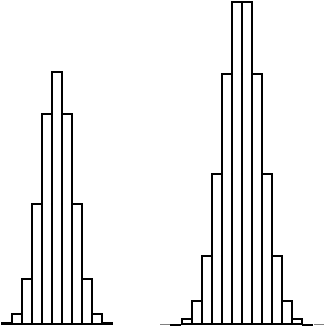
\includegraphics[scale=0.5]{FiguresMaths/ProbaGaussianDistribution}
        \caption{Histograms of the binomial coefficients in the $10$th row (left) and the $15$th
         row (right) of Pascal's triangle, with the entries corresponding to
         $\displaystyle {n \choose 0} = 1$ deleted.
         The scale of the righthand histogram is 1:20.}
        \label{fig:gaussiandistribution}
\end{center}
\end{figure}

\index{binomial distribution} \index{binomial distribution!mean}
\index{binomial distribution!variance} \index{binomial distribution!standard deviation}

The histograms in Fig.~\ref{fig:gaussiandistribution} are---when the entries 
corresponding to $\displaystyle {n \choose 0} = 1$ are restored---instances of the
familiar Bell curve of a {\em binomial (probability) distribution}.

\medskip

Before we discuss probability distributions, we should understand why
they are important.  In a word, distributions give us a global
perspective on very long (possibly infinite) sequences of events.

\subsection{Summarizing Sequences of Events by a Single Number}
\label{sec:single-statistic}
 

**HERE


**HERE

\index{normal distribution} \index{normal distribution!mean} \index{Gaussian distribution}
\index{normal distribution!variance} \index{normal distribution!standard deviation}

discrete versions of the
familiar Bell curve of a 
{\em normal}, or, {\it Gaussian} probability distribution.  
(The word ``normal" in this context emphasizes that these distribution are defined by their ``norms", namely, 
their means and variances.) Although our focus in this text is entirely on {\em discrete} 
mathematical phenomena, it is important to recognize concepts and insights that 
emerge from the {\em continuous} versions of these phenomena.  A (continuous) normal 
distribution is one whose probability frequency function has the form
\[ f(x) \ = \ \frac{1}{\sqrt{2 \pi} \sigma} \ e^{\frac{(x - \mu)^2}{2 \sigma^2} } \]
In this formula: $\mu$ is the {\it mean} of the distribution, and $\sigma^2$ 
(resp., $\sigma$) is its {\it variance} (resp., its {\it standard deviation}).  Indeed, as is clear
from the formula, parameters $\mu$ and $\sigma$ {\em specify} each individual normal 
distribution.

Here are a few noteworthy features of discrete and continuous normal distributions.
\begin{itemize}
\item
In the {\em discrete} version of the concept:
  \begin{itemize}
  \item
In common with the underlying binomial coefficients
\[ \left\{ {n \choose k} \ | \ k = 0, 1, \ldots, n \right\} \]
the distribution has a single maximum when $n$ is even but {\em two}
maxima when $n$ is odd.

  \end{itemize}

In the {\em continuous} version of the concept:
  \begin{itemize}
  \item
As a cultural note, the normal probability frequency function involves two of the
fundamental constants of mathematics: $e$ and $\pi$.
  \end{itemize}
\end{itemize}

\index{probability!distribution function} \index{probability!cumulative distribution function}

In addition to the point-wise information that a probability frequency function yields, we are
often interested in the {\em cumulative} information yielded by the 
{\it (cumulative) distribution function}\footnote{Mathematicians usually refer to function $F$
simply as a distribution function; statisticians usually add the qualifier ``cumulative".}~$F$ 
on $S$, which is defined as follows for $x \in S$:
\[ F(x) \ = \ Pr[X \leq x] \]
In discrete settings, we can redefine $F(x)$ as a summation:
\[ F(x) \ = \ \sum_{y \leq x} \ f(y) \]

{\Arny Examples .. maybe this is the place to define and exemplify the normal distribution
and the exponential distribution?}



\section{Statistics: The Art of Summarization}
\label{sec:statistics}
 
 You have a large corpus of numerical data which has been generated by some manner of
 experiment.
 
\bigskip
 
 \noindent \fbox{
 \begin{minipage}{0.95\textwidth}
Such corpora of  numbers are generated, e.g., when one measures the results of some process
or when one observes some natural or artificial phenomenon.
\begin{enumerate}
\item
An example of the former situation is a Physics 101 Lab experiment that empirically develops an  
estimate of the value of the gravitational force by having students repeatedly drop a ball of known 
mass and time the moment of the ball's impact  with the earth.

\item
An example of the latter situation is an observational experiment that records over fixed periods 
of time the percentage of births in which the newborn has a specific gender.
\end{enumerate}

The second of these examples actually played a significant role in the development of statistics 
and its operational methodology.

\smallskip

\index{Arbuthnot, John} \index{Laplace, Pierre Simon}
The curiosity of the British polymath John Arbuthnot was piqued by the popular belief that males
occur more often than females among newborns.  In an effort to determine the truth or falsity of
this belief, Arbuthnot studied an archive reporting on births in London in the 82-year period
1629--1710.  As reported in his paper,  ``An argument for Divine Providence taken from the 
constant regularity  observed in the births of both sexes" ({\it Philosophical Transactions} of 
the Royal Society, 1710), Arbuthnot observed results such as the following: In 1629, there were 
5218 males born, versus only 4683 females; and in 1710, the corresponding numbers were
7640 versus 7288.  In fact, much to his surprise, the archives exposed a consistent surfeit of
male births over females!  Roughly a century later, the French mathematician Pierre Simon 
Laplace---who, in fact, invented much of the mathematics relating to probability and 
statistics---calculated that male births exceeded female births in the proportion of about
22 to 21 (reported in Laplace's celebrated {\it Essai philosophique sur les probabilit\'{e}s}, 1814).

\smallskip

Interestingly the gender imbalance in births can still be observed today---and the reason for
the imbalance has not yet been clearly identified.

\smallskip

We discuss the technicalities of Arbuthnot's observational experiment a bit later.
\end{minipage}
 }
 
\bigskip
 
The sheer volume of data in the corpus makes it impossible to understand the phenomenon 
being studied.  You really need to summarize them 
in a manner that will give a reliable summary of the import of the data.  The field of statistics provides well-studied approaches to this important challenge.
 
 \medskip
 
 \noindent \fbox{
 \begin{minipage}{0.95\textwidth}
 Our very informal introduction to the field of statistics would be considered irreverent---perhaps
 even blasphemous---to many practitioners of this field.  But, it does provide a reasonably
 accurate way to begin thinking about the field.
 \end{minipage}
 }
 
 \medskip
 
 \index{experiment!trial}  \index{experiment!outcome}  
 \index{experiment!probability of an outcome}
 \index{experiment!frequency of an outcome}
There are two complementary ways to provide information about the data which one might obtain,
say, from an extensive experiment.  We illustrate these via the trivial experiment of rolling a
(possibly biased) $6$-sided die $n$ times.  Within the context of discussing such an experiment,
one typically refers to each roll of the die as a {\it trial} and to the number observed from the roll
as an {\it outcome}.  When discussing this experiment, we can associate with each possible
outcome $x \in \{1,2,3,4,5,6\}$:
\begin{itemize}
\item
the {\em probability} of $x$ occurring.  In this scenario, one thinks of the $n$ outcomes as a
{\em multiset} $S$, and one associates with outcome $x$ the probability, $m/n$, of achieving
outcome $x$ when randomly drawing an element from $S$.
\item
the {\em frequency} with which $x$ occurs in the sequence of outcomes; for instance, $x$ may
occur $m$ times throughout the $n$ rolls.  One typically uses a {\em frequency function} $f$ to
expose this kind of information---noting that $f(x) = m$.
\end{itemize}
Note that the frequency approach does not explicitly mention the number of trials $n$, while
the probability approach does.  As we proceed with our discussion of statistics, we repeatedly
use this die-rolling experiment for illustration.  

\index{Law of Large Numbers} \index{fair} \index{unbiased}
Keep in mind that in the ideal world of probabilities, all six outcomes are equiprobable, hence, 
each has probability $1/6$.  The field of statistics operates in the real world, hence must 
account for the fact that experimental outcomes only approximate the ideal mathematical world.  
The {\it Law of Large Numbers}, which we discuss later, is a theorem that guarantees that over 
``sufficiently long" periods of time, the real world becomes a progressively closer approximation 
to the ideal. In fact, this Law underlies the entire endeavor of ``quality control": if we continue to 
observe that our die produces outcome $3$ inordinately often over a ``sufficiently long" 
experiment, then we conclude that the die is not {\em fair}, or, {\em unbiased}!  (The terms
``fair" and ``unbiased" are synonyms.) Elements of the theory of statistics that go way beyond 
the scope of this text develop tests that determine when an experiment is ``sufficiently long" to 
determine whether our die is unbiased.  Of course, such a determination is not absolute---it
draws its conclusions within some {\em confidence level}.
\index{confidence level}

With this introduction, we now embark on our introduction to statistics.  We stress that this
field has developed and deployed immensely sophisticated mathematical and
computational tools.  We wish here only to given the reader a taste of what the field is
about, so we strive only to hint at its goals and methodology.  We refer the readers to sources
such as \cite{Hoel58} (which focuses on the mathematical aspects of the field) and 
\cite{Bremaud17}  (which provides a comprehensive introduction) for two rather differently
focused comprehensive introductions to this important field.

\section{``Doing" Statistics}
\label{sec:doing-statistics}


The person who wants to discover truth by ``doing" statistics has two primary tools:
\begin{itemize}
\item
{\em experimentation}, which gives one a tunable approximation to how the real world 
operates.

The tunability comes from one's freedom to design the experiments and to decide how
many trials to perform.

\item 
{\em summarization} of the observed outcomes of the experiments, in a manner that 
enables to draw inferences about the real world.
\end{itemize}
Note the role that the Law of Large Numbers plays here by ensuring that performing
more trials yields experimental results that more closely resemble reaity


\ignore{************
Statistics is complementary to probability theory in a sense that can be illustrated by the 
example of tossing a $2$-sided coin.  In this case, the random variable $X$ varies over the set
$\{0,1\}$ (as an encoding of the set $\{\mbox{\sc heads, tails}\}$).  Say that one tosses the
coin $n$ times.  Probability theory captures one element of the ``truth" of the experiment by 
reporting the proportion of tosses in which variable $X$ assumes each of its possible outcomes.  
Statistics captures a somewhat different element of truth by reporting results such as the 
observed {\em average} value observed---even if this average never actually occurred!  Thus,
if $n=100$ and the coin is observed to come up {\sc heads} on $52\%$ of the tosses, then one
might infer that the probability 

strives focuses on the 
frequencies of the various possible outcomes; probability theory focuses on the relative ratios 
of the possible outcomes.  
***************}




******************
**HERE

I have now gotten into Sec 11.4.2.  My proposals:

1. We move Fig. 11.8 to illustrate the def?n of frequency function (with a very different, statistics-based, caption) and that we add the cumulative version of 11.8 as Fig. 11.9.

2. Once we have step 1, it is natural to introduce the normal distribution ? emphasizing that ?normal? means ?coming from a norm?, not anything to do with the vernacular use of ?normal? as ?usual?.

3. While we do this, I propose that we add the exponential distribution also ? with analogs of Figs. 11.8 and 11.9.  Our friend YR suggests over a glass of wine that the normal and exponential distributions are all one needs for empirical work :)

4. Now, we move to Empirical Reasoning.  The subsections will consist of
(a) births of boys and girls
(b) some mention of testing (very superficial)
(c) the Loi des grand nombres: (i) both in the weak and strong forms; (ii) with no proof!  (The only proofs I have seen are way beyond early students.)

WHAT WILL THIS MISS?
***********************

\subsection{Using statistics to make predictions}
\label{statistical-predictions}

The Law of Large Numbers


{\Denis I copied the two following paragraphs from the existing text (written a long time ago by you...}

Most students whose interest tend to the empirical will likely ``do"
statistics with the aid of apps, rather than by explicitly writing
programs that perform the required calculations.  That said, all
students should understand the crucial notion of {\em random variable}
and should be conversant with the most common statistical
distributions.  ``Conversant" in this context should include complete
understandings of the (low-numbered) moments of {\em at least} the
{\em uniform} and {\em exponential} distributions.  They should know
how to compute, say, the means and variances of various distributions
— and, most importantly, they should {\em understand} the sense in
which the variance of a distribution give {\em important} information
that is not available from the mean.  All of this is prerequisite to
rigor in experimentation.

\subsection{The Elements of Empirical Reasoning}

Empirical reasoning does not convey the certitude that formal
reasoning does.  Students should understand how to craft experiments
in a way that collects the ``right'' data.  The should then be
able---perhaps just with statistical packages---to interpret the
results they collect and to understand what conclusions are
justifiable.  {\em It is essential that all students understand the                  
  distinction between {\em positive correlation} and {\em causation}!}
(Most of the public would seem to flunk that test.)

In order to satisfy the preceding demands, students should understand
enough about statistics---including definitions and meanings related
to distributions and their moments---to understand what conclusions
can be made based on experimental results, and to understand how to
describe conclusions in a way that is supported by the statistics.


\subsection{An old story}

The following example reports one of the oldest statistical problem.

{\Arny I do not understand the point of this story.  Is the point that arguing using statistics is
difficult? misleading?  Maybe the point is that the underlying probability (of the birth of a boy)
is {\em not} ${1 \over 2}$.  Where does this fit in to our understanding of statistics?}


{\Arny In the next subsections you seem to be trying to illustrate the Law of Large Numbers --- but
you have not yet defined it.  More importantly, you have not defined the notions that underlie the
Law}

In his paper,
\textit{An argument for divine providence taken from the constant regularity observed in the births of both sexes}
appeared in Philosophical transactions, 1710, 
% As pointed out by Bernard Ycart, this is the first known statistical reasoning~\cite{websiteBernard}.
John Arbuthnot studied the number of births over an archive of 82 years and draw the proportions of boys and girls
in London (UK) from 1629 to 1710. 
In 1629, there was  5218 males for only 4683 females and in 1710, 7640 against 7288. 
 
The observation was systematic, and the result was surprising: there are always more male births than female births
(in the proportion of about 22 to 21 as pointed out some time later by Pierre Simon Laplace in his 
\textit{Essai philosophique sur les probabilités} in 1814). 
Notice that it is still true today, and the reason has not yet been clearly identified...


**HERE
We return to John Arbuthnot and his study of gender bias in human births.

..

Here the reasoning done by Arbuthnot:
if the births are random, then the probability to have more boys than girls should be equal to 
$p=(\frac{1}{2})^{n}$ for $n$ years of observation.
He succeeded to get the records for the last $82$ years, this means $p \rightarrow 0$.
In other word, there is a quasi null probability to have more boys than girls, which contradicts the observations. 

He looked at this problem by using an analogy with 2 face dices labelled Male and Female
(Today, we will rather talk about tossing coins). 
\medskip

The sketch of the statistical proof is as follows:

Assuming that the events (births) are independent and equiprobable,
%, and there is no difference between boys and girls.
the experience is taken over a long period (82 years), it shows that the probability to have more boys is very tiny and
tends to zero. 
Thus, the hypothesis of an even repartition is false: there are more boys than girls!
\medskip

This is an illustration of the large number law, which says that the probability can be interpreted 
as a limit of experimental measures (frequency of occurence of an event). 
\bigskip

\noindent \fbox{
\begin{minipage}{0.95\textwidth}
Probability or Statistics?
Two faces of the same thing!

Repeating a random experience more and more gives a better (accurate) value
of the relative frequency of the events, which tends to a limit. 

This is another way to look at the probability that an event occurs. 
\end{minipage}
}
\bigskip

The next section is devoted to give more details on this important law.


\subsection{The Law of Large Numbers} 
\label{subsec:LawLargeNumbers}
%\textit{Loi des grands nombres}}

{\Denis add ref: Jocobi Bernoulli, Ars conjectandiopus posthumum}

The former traces of the large numbers law are in a book from Jakob von Bielfeld in 1767.
Later, with the emergence of the probability theory and in particular via the swiss mathematician Jacques Bernoulli
and his nephew Nicholas who finished the work of his uncle when he died, 
the law of large numbers was given as a theorem for describing the result of performing the same experiments
 a large number of times. 
 According to this result, the average of the results obtained from a large number of experiences is close 
 to the expected value. 
For instance, a single roll of a die produces evenly one of the numbers 1 to 6.
Thus, the According to the law, if a large number of dice are rolled, the average of their values 
is likely to be close to the value $\frac{1+2+3+4+5+6}{6}=3.5$.
The precision is increasing with the number the dices are rolled. 

\bigskip

Let consider a hat containing white and black balls.
We will discuss two variants: first, the number of balls is known and second, it is not.

\begin{itemize}
\item If the proportion is known (say for instance 300 white balls and 200 black balls
(thus, $60\%$ of white and $40\%$ of black).

Clearly, there is more chance to get a white than a black.
But the Loi des grands nombres tell us a bit more: the probability to get a white is close to $60\%$
if we are drawing a ball a large number of times and putting it back in the hat.

If we are doing only one trial, the result is simply $1$ or $0$ (if I get a black or not)...
How many trials do we have to do to be sure that the probability is $60\%$?
For instance, draw ten balls, are we sure to obtain $6$ white balls? What about $100$ or $1000$?
\item If the number of balls is not known.
The experience consists in determining the probability to draw a white ball without knowing 
We proceed as before:
draw a ball, note his color and put it back in the hat, and do it again and again...
%(then, the proportion of white/black balls remains unchanged)

The loi des grands nombres will provide the answer (the limit) for an infinite number of trials.
If we want to be sure to obtain the result with a precision of $1\%$,
how many trials do we have to do to get a probability in the interval $(59.9,60.1)$?
\end{itemize}

\medskip

\noindent \fbox{
\begin{minipage}{0.95\textwidth}
In the loi des grands nombres, called also the \textit{golden theorem} (Th\'eor\`eme d'or) by Jacques Bernouilli,
large numbers refer to the convergence of the frequency of occurrence of an experience to a limit, which is the probability
that the event occurs. 

The Loi des grands nombres gives also a solution to the problem of how many trials are needed to obtain a given
precision...

\end{minipage}
}
\bigskip

{\Denis I think we should conclude by the Loi normale and the gaussian distribution. }

The story is very interesting, it has been the main work of Abraham de Moivre (1667-1754), 
which studied the sum of the terms that appear in the binomial formula of Newton when the power $n$ is large.
His idea was to link with the probability of an event $n$ being the number of times this event occurs.

The binomial expression is:

$(1+x)^n = \sum_{k=0,n-1} {n \choose k} x^k = (1+x)(1+x)\ldots(1+x)$

in each of the $n$ factors $(1+x)$, choose $1$ or $x$, we obtain the coefficient of $x^k$.

\medskip




\section{Beyond the Basics}

As students are introduced to modern topics within computing, whether
at the level of a Computing Literacy course or a post-core technical
course, they will have to master a variety of more specialized topics
that combine pieces of the elements we have discussed in this essay.
While these topics are beyond the level of generality aimed at in this
essay, some may be appropriate prerequisites to programs that have
some specialized foci.
\begin{itemize}
\item
Issues relating to {\em clustering} find application in applications as
diverse as: {\em linear-algebraic computations}, {\em data mining},
{\em design and layout of digital circuitry}.

\item
Issues building on {\em graph separation/decomposition} are
encountered when studying: {\em linear-algebraic computing}, {\em
  fault-tolerant design}, {\em load balancing}.

\item
Many issues relating to {\em fault/failure tolerance} and {\em data
  analytics} benefit from study using {\em random walks} (at least in
one dimension).

\item
Many useful ideas regarding the {\em encoding and manipulation of
  data} can be gleaned from the elements of {\em information theory}
and {\em computer arithmetic}.
\end{itemize}
The preceding list is really endless.  Hopefully readers will be
inspired by our few examples to compile a longer version that is
appropriate for their particular environments.

